
\documentclass[skorowidz,autorrok,backref,xodstep,oswiadczenie]{wmimgr}

\usepackage{listings}
\usepackage{color}
\usepackage{alltt}
\usepackage{floatrow}
\usepackage{hyphenat}
\usepackage{url}
\usepackage{mathtools}
\usepackage{algorithmic}
\usepackage[chapter]{algorithm}
\usepackage{graphicx}

\newcommand\dbr{\discretionary{}{}{}}


% Opcjonalnie identyfikator dokumentu (drukowany tylko z włączoną opcją `brudnopis'):
\nrwersji {0.1}

% Dane autora(ów):
\author   {Wojciech Chojnacki}
\nralbumu {369971}
\email    {s367791@wmi.amu.edu.pl}

% Tytuł pracy:
\title    {Hierarchiczny Model Podziału Obiektów}

% Kierunek, tj. katedra/instytut promotora:
\kierunek {Informatyka}

% Rok obrony:
\date     {2013}

% Jeżeli nie podano miejsca zostanie wpisany `Sopot'
\miejsce {Poznań}

% Tytuł naukowy, imię i nazwisko promotora:
\opiekun  {dr Wojciech Kowalewski}

%
% Miejsce na deklaracje własnych poleceń:
\newcommand{\filename}[1]{\texttt{#1}}

% Cytowanie przez numer (standard):
%\bibliographystyle{plain}
%
% Jeżeli cytowanie autor-rok to np.:
\bibliographystyle{papalike}
%
% Inne sposoby
%\bibliographystyle{abbrv} %% standard
%\bibliographystyle{acm} %% ACM transactions...
%\bibliographystyle{elsart-harv} %% dziwaczny %%

%%% zakomentuj \iffalse ... \fi (ostatnie, zaznaczone //pdfscreen) jeżeli chcesz włączyć pakiet pdfscreen:
\def\SITI{SI/TI} %%%
\def\ISTI{SI/TI} %%%
\def\UTAUT{UTAUT} %%%

\begin{document}

%%
%%\nocite{beebe,p.perl} %% dołącza niecytowane
\nocite{*} %% ** dołącza wszystko **

% Streszczenie
\begin{abstract}

Praca opisuje metodę podziału trójwymiarowej siatki obiektu z~użyciem \emph{Diagramu Voronoi}. Przedstawiona została teoretyczna definicja i~właściwości zarówno diagramu, jak i~powiązanej z~nim \emph{Triangulacji Delaunay}. Omówione zostały ich najczęstsze zastosowania i~metody obliczania. Ponieważ celem pracy jest operowanie na~obiektach~3D, przedstawione zostały istotne różnice pomiędzy przypadkami dwu-~i~trójwymiarowymi. Pokazane zostały istotne szczegóły implementacyjne tych zagadnień zastosowane w~dołączonej do~tej pracy aplikacji stworzonej z~wykorzystaniem technologii C++, OpenGL oraz QT4. Ostatni rozdział przedstawia możliwości dalszego rozszerzania omówionego tematu.

\end{abstract}

% Tytuł/spis treści
\maketitle

%
% Spis tabel (jeżeli jest potrzebny):
%\listoftables
%
% Spis rysunków (jeżeli jest potrzebny):
\listoffigures

%
% Skorowidz (opcjonalnie)
% \printindex

%
% Wstęp
\chapter{Wstęp}

W~pierwszym rozdziale pracy zarysujemy jej temat, przedstawimy jego genezę oraz potencjalne, praktyczne zastosowania.

\section{Sformułowanie Problemu}

Tematem niniejszej pracy jest opracowanie metody podziału obiektów na~części. Metoda powinna działać w~czasie rzeczywistym, a~wynik~jej działania powinien być zbliżony do~realistycznego. Przygotowana implementacja powinna być modularna i~pozwalać na~łatwe dopasowanie jej do~różnorodnych rendererów oraz silników fizycznych. Dodatkowo aplikacja powinna umożliwiać podstawową parametryzację podziałów, zapewniając co najmniej możliwość określenia ilości uzyskiwanych fragmentów.

\section{Geneza Tematu}

Początkowo tematem pracy miała być dynamika materiału sypkiego przedstawiona jako szczególny przypadek dynamiki płynów. Jednak w~miarę jego badania okazało się, że~jego istotnym uzupełnieniem jest zagadnienie jego uzyskiwania. Podział jednolitej bryły na~fragmenty jako dopełnienie zachowań fizycznych dużej ilości drobnych obiektów okazał się na~tyle rozległy i~interesujący, że~praca została ograniczona tylko do~tego zagadnienia. Mimo to, pierwotny temat nie został całkiem zarzucony i~pewne możliwości dalszego rozwoju zostały przedstawione w~ostatnim rozdziale niniejszej pracy.

\section{Zastosowania}

Przedstawione w~tej pracy metody mogą zostać użyte w~modelowaniu w~czasie rzeczywistym, np. w~grach komputerowych, ale nie tylko. Można użyć ich także we~wszelkiego rodzaju symulacjach zniszczeń, oraz modelach wymagających rozpadu obiektów do~materiału sypkiego. Przykładem takiego zastosowania może być symulacja rozmywania wałów przeciwpowodziowych.

Stosowane obecnie rozwiązania podziałów w~czasie rzeczywistym, zwłaszcza te~nie nastawione na~realistyczne odwzorowanie fizyki, najczęściej korzystają ze~statycznych podziałów obiektów. Prowadzi to~do~takich problemów, jak powtarzalność wyników, nienaturalne zachowanie (nierealistyczny rozpad względem punktu kolizji) oraz niezachowanie objętości.

Z~drugiej strony aplikacje wymagające zaawansowanej fizyki i~zbliżone do~rzeczywistości, nie wymagające jednak pełnego odwzorowania, mogą skorzystać z~przedstawionej tu~metody, aby efektywnie realizować dynamiczne, losowe podziały.

\chapter{Diagram Voronoi}

W~niniejszym rozdziale wprowadzone zostanie pojęcie \emph{Diagramu Voronoi}, znanego także jako \emph{Teselacja Dirichleta}. Omówione zostaną najważniejsze właściwości diagramu, jego praktyczne zastosowania oraz metoda tworzenia w przestrzeni dwuwymiarowej.

\section{Definicja}

Opiszmy odległość euklidesową między punktami $p$ i $q$ jako funkcję $dist(p,q)$. Na płaszczyźnie otrzymujemy
\begin{equation}
dist(p,q) := \sqrt{( p_{x} - q_{x} )^2 + (p_{y} - q_{y})^2}
\end{equation}

Niech $P:=\{ p_{1},p_{2},...,p_{n} \}$ będzie zbiorem punktów na~płaszczyźnie euklidesowej $E$. Zbiór ten nazywamy zbiorem centrów. \emph{Komórką Voronoi} dla punktu~$p_{i}$ ze~zbioru~$P$ nazywamy zbiór punktów znajdujących się bliżej punktu $p_{i}$ niż jakiegokolwiek innego punktu ze~zbioru~$P$
\begin{equation}
Vor(p_{i}) := \{ x \in E | \forall q \in P, q \neq p_{i}, dist(x,p_{i}) < dist(x,q) \}
\end{equation}

\begin{figure}[ht!]
\centering
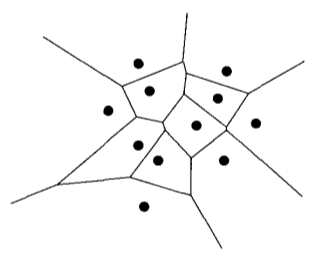
\includegraphics[width=70mm]{images/voronoi1.png}
\caption{Przykładowy diagram Voronoi. Źródło \cite{geometria}}
\label{voronoidiagram}
\end{figure}

W~zależności od kontekstu \emph{Diagramem Voronoi} nazywać będziemy zbiór komórek Voronoi utworzonych na~podstawie punktów ze zbioru~$P$, lub też graf o~wierzchołkach i~krawędziach utworzonych przez punkty będące w~równej odległości od dwóch lub więcej punktów ze~zbioru~$P$.

\section{Właściwości}

Rozważmy pojedyńczą komórkę diagramu. Niech $h(p,q)$ będzie otwartą półpłaszczyzną utworzoną przez prostą prostopadłą do~odcinka~$\overline{pq}$ dzielącą go na równe połowy, zawierającą punkt~p, nie zawierającą dzielącej prostej
\begin{equation}
h(p,q) := \{ x \in E | dist(x,p) \leq dist(x,q) \}
\end{equation}

Zauważmy, że komórkę możemy opisać jako przekrój $n-1$ półpłaszczyzn
\begin{equation}
Vor(p_{i}) := \bigcap_{1 \leq j \leq n, j \neq i} h(p_{i},p_{j})
\end{equation}
a więc jest wielokątnym, wypukłym oraz potencjalnie nieograniczonym obszarem płaszczyzny utworzonym przez conajwyżej $n-1$ wierzchołków i $n-1$ krawędzi. Krawędzie diagramu mogą być zarówno odcinkami, jak i półprostymi. O ile nie wszystkie punkty $p_{i} \in P$ są współliniowe, diagram nie zawiera krawędzi będących prostymi.

Zdefiniujmy $Cp(q)$ jako \emph{największy, pusty okrąg o środku w punkcie $q \in E$} nie posiadający w swoim wnętrzu żadnego punktu ze zbioru $P$. Jeżeli $p \in Cp(q)$ to punkt $p$ lezy na tym okręgu.
Obserwując, że wierzchołki diagramu znajdują się w równej odległości od trzech lub więcej punktów, możemy określić ich zbiór jako
\begin{equation}
P_{v} := \{ x \in E | \exists p,q,r \in P, p,q,r \in Cp(x) \}
\end{equation}

Punkty krawędzi diagramu znajdują się w równej odległości od dwóch centrów, lecz w większej odległości od jakichkolwiek innych punktów. Tak więc krawędź diagramu pomiędzy punktami $p,q \in P$ określamy jako
\begin{equation}
Ve(p,q) := \{ x \in E | \forall r \in P, p \neq r, q \neq r, p,q \in Cr(x), r \notin Cr(x) \}
\end{equation}

\begin{figure}[ht!]
\centering
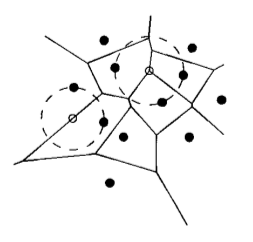
\includegraphics[width=70mm]{images/voronoi2.png}
\caption{Punkty krawędzi oraz wierzchołki. Źródło \cite{geometria}}
\label{voronoicircles}
\end{figure}

Komórki Voronoi o centrach $p,q \in P$ określamy jako \emph{przyległe}, jeżeli zbiór $Ve(p,q)$ jest niepusty.

\section{Zastosowania}

Ze względu na swoje właściwości Diagram Voronoi ma wiele różnorodnych zastosowań. Wykorzystywany jest on między innymi w
\begin{itemize}
\item
Wieże obserwacyjne - aby~szybko wykrywać pożary lasów, rozstawiane są w~nich wieże obserwacyjne. Używając lokacji wież jako centrów budujemy diagram wyznaczający obszary obserwowane przez każdą wieże. Dzięki temu leśnicy są~w~stanie określić, które wieże posiadają zbyt dużo lub~zbyt mało odpowiedzialności oraz które części lasu wymagają lepszego pokrycia.
\item
Punkty usługowe - budując sieć punktów usługowych (np.~poczta, supermarkety, pizzerie) Diagram Voronoi pozwala określić obszar obsługiwany przez dany punkt. Dzięki temu można zdecydować, czy~uzasadnione jest~istnienie danego punktu usługowego lub~też~czy~dane miejsce zapewni wystarczająco dużo klientów w~okolicy aby~opłacało się~postawić tam~nowy sklep. Aby móc zastosować diagram w~jego podstawowej formie zdefiniowanej w~tym~rozdziale, potrzebne są~dodatkowe założenia, takie, jak~równy koszt usługi w~każdym punkcie, lub~też~koszt podróży liniowo proporcjonalny do~odległości od~punktu usługowego.
\item
Terytoria zwierząt - znając położenie legowisk osobników (lub~też~całych stad) danego gatunku możemy modelować ich terytoria, obszary łowne, itp.
\item
Ścieżki robotów - znając rozkład przeszkód na~danym terenie robot może wygenerować mapę bezpiecznych ścieżek utworzonych z~krawędzi diagramu, w~którym przeszkody są~centrami komórek.
\item
Epidemiologia - stosując Diagram Voronoi można modelować rozprzestrzenianie się~choroby w~danej populacji
\item
Sieci bezprzewodowe - na podstawie diagramu mozna stwierdzić jak duże jest obciążenie punktów dostępowych w sieci obejmującej dany teren
\end{itemize}
Diagram wykorzystywany jest także w górnictwie, klimatologii i innych dziedzinach.

\section{Obliczanie Diagramu}

Jak zauważyliśmy w~sekcji \emph{Właściwości}, komórka diagramu jest~przecięciem zbioru półpłaszczyzn. Obserwacja ta~pozwala utworzyć pojedyńczą komórkę w~czasie~$O(n \log{n})$, przy zastosowaniu algorytmu przecinania półpłaszczyzn opisanego w~\cite{geometria}. Złożoność obliczeniowa dla~całego diagramu wynosi~$O(n^2 \log{n})$.

Optymalnym algorytmem obliczania diagramu Voronoi jest \emph{algorytm Fortune'a} obliczający wszystkie komórki w~czasie~$O(n \log{n})$. Stwierdzenie to opiera się na fakcie, że problem sortowania $n$ liczb rzeczywistych można sprowadzić do tworzenia diagramu Voronoi, a więc jego obliczenie zajmuje najwyżej $\Omega(n \log{n})$ czasu.

\subsection{Algorytm Fortune'a}

\emph{Algorytm Fortune'a} buduje diagram poprzez skanowanie płaszczyzny poziomą prostą. Zbiera on~informacje o~przecięciu już~wygenerowanej struktury z~prostą skanującą. Informacja ta~zmienia się~tylko w~określonych momentach zwanych \emph{zdarzeniami punktowymi}.

Podstawą dla~rozpoczęcia algorytmu jest~zbiór $P = \{p_{1},p_{2},...,p_{n}\}$ punktów na~płaszczyźnie~$E$. Płaszczyzna ta~skanowana jest prostą $l$ przesuwającą się z~góry na~dół. Największym problemem w~budowaniu komórek jest fakt, że~na~ich~kształt wpływają nieprzeskanowane jeszcze punkty poniżej prostej. Kiedy prosta dociera do~komórki $Vor(p_{i})$ nie~posiada ona jeszcze informacji o~punkcie~$p_{i}$. Dlatego też w~praktyce stosuje się~odrobinę inne podejście. Zamiast badać przecięcie diagramu z~prostą skanującą~$l$, zbierane są~informacje o~tych punktach~$q \in E$ powyżej prostej, na~które nie~może już~mieć wpływu żaden punkt~$p_{i}$ znajdujący się~pod~nią.

\begin{figure}[ht!]
\centering
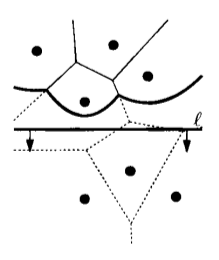
\includegraphics[width=60mm]{images/voronoi3.png}
\caption{Przykład plaży. Źródło \cite{geometria}}
\label{voronoibeach}
\end{figure}

Otwartą półpłaszczyznę powyżej prostej~$l$, na~której znajdować będą się~wyrysowane już~komórki, określać będziemy symbolem $l^{+}$. Musimy zbadać, które~fragmenty diagramu powyżej~$l$ nie~zostaną już~zmienione przez centra poniżej. Odległość punktu~$q \in l^{+}$ od~każdego~$p_{i}$ poniżej~$l$ jest większa niż~jego odległość od~prostej~$l$. Dlatego też~najbliższe centrum dla~punktu~$q$ musi znajdować się~ponad~$l$ jeżeli odległość punktu od~jakiegokolwiek centrum powyżej~$l$ jest~mniejsza od~odległości od~prostej~$l$. Obszar punktów będących bliżej punktu~$p_{i}$ niż prostej~$l$ ograniczony jest parabolą $\beta_{i}$. Linia złożona z~parabolicznych łuków nazywana jest~\emph{plażą}. Można ją~wyrysować funkcją, która dla~każdego~$x$ wybiera najmniejszą wartość ze~wszystkich paraboli~$\beta_{i}$.

Parabola~$\beta_{i}$ może zostać użyta do~utworzenia kilku rozłącznych fragmentów plaży. Punkty znajdujące się~na~przecięciach parabol wyrysowują krawędzie diagramu. Linia plaży istotnie zmienia się~w~przypadku wystąpienia jednego z~dwóch typów zdarzeń: pojawienie się~nowej paraboli oraz zredukowanie udziału paraboli do~pojedyńczego punktu.

\subsection{Zdarzenia}

Pojawienie się~nowej paraboli~$\beta_{i}$ możliwe jest jedynie przez natrafienie prostej $l$ na punkt~$p_{i} \in P$. Pojawia się~wtedy zdegenerowana parabola o~zerowej szerokości połączona z~plażą. Wraz z~przesuwaniem się~prostej~$l$ parabola~$\beta_{i}$ rozszerza się. Miejsca jej~przecięcia z~poprzednią plażą rysują nową krawędź diagramu, która~nie~jest jeszcze połączona z~jego resztą. Fragment paraboli~$\beta_{i}$ znajdujący się~poniżej poprzedniej plaży staje się~jej nowym fragmentem tworząc nową plażę. Można z~tego wywnioskować, że~plaża może składać się~z~co~najwyżej~$2n-1$ parabolicznych fragmentów.

\begin{figure}[ht!]
\centering
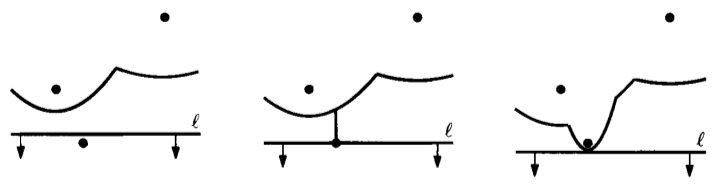
\includegraphics[width=150mm]{images/voronoi4.png}
\caption{Pojawienie się nowej paraboli. Źródło \cite{geometria}}
\label{voronoinewarc}
\end{figure}

Drugim typem zdarzenia wpływającym na~kształt plaży, a~przez to~diagramu, jest~zniknięcie fragmentu plaży. Niech~$\alpha'$ będzie zanikającym łukiem, a~$\alpha$ i~$\alpha''$ łukami sąsiadującymi z~$\alpha'$ przed jego zniknięciem. Łuki $\alpha$ i~$\alpha''$ nie mogą należeć do~tej~samej paraboli~$\beta_{i}$, tak więc łuki~$\alpha$, $\alpha'$ oraz~$\alpha''$ tworzone są poprzez trzy różne centra~$p_{i}$, $p_{j}$ oraz~$p_{k}$ należące do~zbioru~$P$. W~momencie, w~którym łuk~$\alpha'$ zanika, parabole~$\beta_{i}$, $\beta_{j}$ oraz~$\beta{k}$ przechodzą przez wspólny punkt~$q$. Punkt~$q$ znajduje się~wtedy w~równej odległości od~prostej~$l$ oraz od~wszystkich trzech punktów, a~więc istnieje okrąg o~środku w~punkcie~$q$, zawierający punkty~$p_{i}$, $p_{j}$ i~$p_{k}$ na swojej krawędzi, oraz nie~zawierający żadnego innego punktu z~$P$ w~swoim wnętrzu. Punkt $q$ jest więc wierzchołkiem diagramu, a~zaniknięcie fragmentu plaży~$\alpha'$ oznacza spotkanie się~dwóch krawędzi diagramu (spotkanie większej ilości krawędzi można sprowadzić do~kilku zdarzeń spotkania dwóch krawędzi).

\begin{figure}[ht!]
\centering
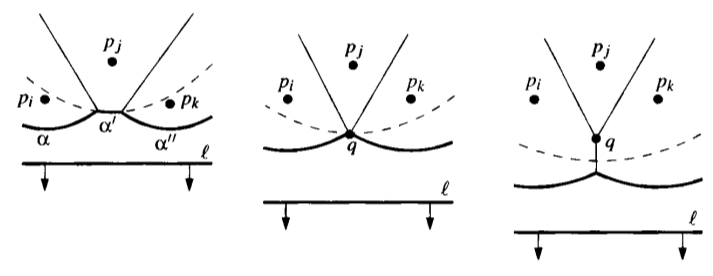
\includegraphics[width=150mm]{images/voronoi6.png}
\caption{Zanik paraboli. Źródło \cite{geometria}}
\label{voronoidelarc}
\end{figure}

\subsection{Struktury Danych}

Kolejnym istotnym elementem algorytmu jest~określenie odpowiednich struktur danych do~przechowywania informacji o~już utworzonych częściach diagramu, kolejce zdarzeń, oraz o~bierzącym stanie prostej (a~w~zasadzie plaży). Proponowane dla nich jest użycie następujących implementacji:
\begin{itemize}
\item
Gotowe elementy diagramu przechowujemy w~strukturze danych opisanej w~\cite{geometria}. Składa się~ona z~listy wierzchołków wraz z~ich~współrzędnymi, listy komórek ze~wskazaniem na~początki łańcuchów krawędzi zewnętrznych i~wewnętrznych, oraz listę krawędzi, opisanych poprzez punkt początkowy, kolejną i~poprzednią krawędź, bliźniaczą krawędź oraz komórkę. Struktury te będziemy zbiorczo oznaczać jako $\mathcal{D}$. Aby po zakończeniu obliczeń dane były spójne, potrzebne jest jeszcze ograniczenie przestrzeni, na której generowany jest diagram.
\item
Do~reprezentowania plaży używane jest~zrównoważone drzewo binarne $\tau$. Jego liście przechowywują informacje łukach należących do~$x$-monotonicznej linii plaży, ułożonych w~kolejności od~lewej. Wewnętrzne węzły drzewa reprezentują punkty załamania plaży. Punkty te~przechowywane są~jako pary punktów~$\langle p_{i}, p_{j}\rangle$, gdzie~$p_{i}$ definiuje lewą parabolę, a~$p_{j}$ prawą parabolę. Dzięki takiej reprezentacji możemy znaleźć łuk znajdujący się~nad nowym punktem w~czasie~$O(\log{n})$ poprzez porównywanie współrzędnej~$x$ węzłów pośrednich i~prostej~$l$ w~ustalonym punkcie czasu.
Każdy liść drzewa $\tau$ przechowuje także wskaźnik do~zdarzenia w~kolejce oznaczającego zanik odpowiedniego łuku $\alpha$. Wskaźnik ten jest pusty, jeżeli łuk nie zniknie, lub wydarzenie nie zostało jeszcze wykryte. Każdy z~węzłów pośrednich posiada wskaźnik na~krawędź z~listy opisanej powyżej, która rysowana jest przez to~przecięcie parabol.

\begin{figure}[ht!]
\centering
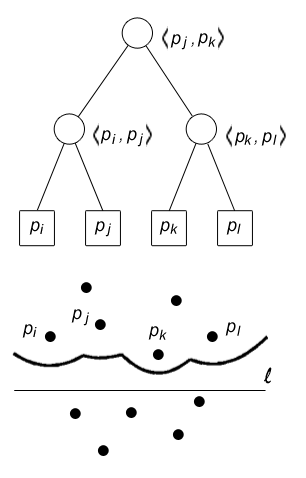
\includegraphics[width=100mm]{images/tree.png}
\caption{Drzewo parabol. Źródło \cite{geometria}}
\label{voronoidelarc}
\end{figure}

\item
Kolejka zdarzeń $Q$ hierarchizuje je~ze~względu na~współrzędną~$y$ jego wystąpienia. Przechowywane są~jedynie przyszłe zdarzenia, które są~już~znane. Dla pojawiania się ~owych łuków, przechowywane są~ich~punkty~$p_{i}$. Dla~znikających łuków przechowywany jest~najniższy punkt z~okręgu ze~wskaźnikiem do~liścia z~$\tau$, który go~reprezentuje.
\end{itemize}

\subsection{Wykrywanie Zdarzeń}

Jak łatwo zauważyć, wszystkie zdarzenia dodawania nowych łuków są~z~góry znane, gdyż są~one powiązane z~punktami~$p_{i} \in P$. Zdarzenia zaniku łuków muszą zostać wykryte.

Podczas skanowania linia plaży zmienia swoją topologiczną strukturę przy każdym zdarzeniu z~kolejki. Może to powodować pojawienie się~na~niej nowej trójki łuków, lub zniknięcie już istniejącej. Algorytm zapewnia, że~dla~każdej trójki łuków mogącej spowodować zanik środkowego z~nich, dodane zostanie odpowiednie zdarzenie do~kolejki~$Q$. W~trakcie wykrywania należy uwzględnić dwa szczególne przypadki: dwa punkty definiowane przez trzy łuki nigdy się~nie~spotkają, oraz zniknięcie całej trójki zanim nastąpi odpowiednie zdarzenie poprzez pojawienie się~pod~nią~nowego łuku.

W~trakcie wykonania algorytmu, po~każdym zdarzeniu z~kolejki~$Q$ sprawdzane są~możliwości wystąpienia nowych i~dodawane do~kolejki. Sprawdzane jest także, czy~dla znikającej trójki nie~zostało dodane zdarzenie do~kolejki, po~czym jest~ono usuwane.

\subsection{Pseudokod}

Bazując na~powyższych ustaleniach można spisać gotowy algorytm. Warto zauważyć, że~po wykonaniu ostatniego zdarzenia plaża jeszcze nie~zanika. Dlatego też pozostałe krawędzie muszą zostać połączone z~prostokątem ograniczającym przestrzeń.

\begin{algorithm}
\caption{$VoronoiDiagram(P)$ \cite{geometria}}
\label{fortune}  % and a label for \ref{} commands later in the document
\begin{algorithmic}
    \REQUIRE $P := \{p_{1}, p_{2}, ... , p_{n}\}$
    \STATE Init $\mathcal{Q, T, D}$
    \WHILE{$\mathcal{Q}$ is not empty}
        \STATE Get event $q$ from $\mathcal{Q}$ with largest $y$-coordinate
        \IF{$q$ is site event for $p_{i}$}
            \STATE $HandleSiteEvent(p_{i})$
        \ELSE
            \STATE Get leaf $\gamma$ from tree $\mathcal{T}$ representing dissapearing arc
            \STATE $HandleCircleEvent(\gamma)$
        \ENDIF
    \ENDWHILE
    \RETURN $\mathcal{D}$
\end{algorithmic}
\end{algorithm}

\begin{algorithm}
\caption{$HandleCircleEvent(\gamma)$ \cite{geometria}}
\label{HandleCircleEvent}
\begin{algorithmic}
    \REQUIRE $P := \{p_{1}, p_{2}, ... , p_{n}\}, \mathcal{Q, T, D}$
    \STATE Delete leaf $\gamma$ representing arc $\alpha$ from $\mathcal{T}$
    \STATE Update internal nodes of $\mathcal{T}$
    \STATE Rebalance tree $\mathcal{T}$
    \IF{$\gamma$ predeccessor and successor points to circle events $q, l$}
        \STATE Remove events $q, l$ from $\mathcal{Q}$
    \ENDIF
    \STATE Add half-edge with centre of circle event $c$ to list $\mathcal{D}$
    \STATE Add two half-edge records for new breakpoint in $\mathcal{D}$
    \STATE Set pointers between new half-edges
    \STATE Link new records with those in $\mathcal{D}$ ending in vertex $c$
    \IF{three arcs with left neighbour of $\alpha$ as middle cause it to disappear}
        \STATE Add circle event $q$ into queue $\mathcal{Q}$
        \STATE Link event $q$ with disappearing arc leaf in $\mathcal{T}$
    \ENDIF
    \IF{three arcs with right neighbour of $\alpha$ as middle cause it to disappear}
        \STATE Add circle event $q$ into queue $\mathcal{Q}$
        \STATE Link event $q$ with disappearing arc leaf in $\mathcal{T}$
    \ENDIF
\end{algorithmic}
\end{algorithm}

\begin{algorithm}
\caption{$HandleSiteEvent(p_{i})$ \cite{geometria}}
\label{HandleSiteEvent}
\begin{algorithmic}
    \REQUIRE $P := \{p_{1}, p_{2}, ... , p_{n}\}, \mathcal{Q, T, D}$
    \IF{$\mathcal{T}$ is empty}
        \STATE Insert site event $p_{i}$ into $\mathcal{T}$
    \ELSE
        \STATE Find arc $\alpha$ vertically above $p_{i}$
        \IF{$\mathcal{T}$ leaf representing $\alpha$ points to circle event $q$}
            \STATE Remove $q$ from $\mathcal{Q}$
        \ENDIF
        \STATE Replace leaf in $\mathcal{T}$ representing $\alpha$ with subtree having leafs for $\alpha', \alpha'', \alpha'''$
        \STATE Store site $p_{i}$ in $\alpha''$ leaf
        \STATE Get site $p_{j}$ from $\alpha$ leaf
        \STATE Store site $p_{j}$ in $\alpha', \alpha''$ leafs
        \STATE Store tuples $\langle p_{j}, p_{i}\rangle$, $\langle p_{i}, p_{j}\rangle$ in new internal nodes
        \IF{$\mathcal{T}$ is not balanced}
            \STATE Rebalance tree $\mathcal{T}$
        \ENDIF
        \STATE Add edge to $\mathcal{D}$ separating $\mathcal{V}(p_{i}), \mathcal{V}(p_{j})$ with newly created breakpoints $\langle p_{j}, p_{i}\rangle$, $\langle p_{i}, p_{j}\rangle$
        \IF{arc triplet with $p_{i}$ as left arc causes middle arc to dissapear}
            \STATE Add circle event $q$ into queue $\mathcal{Q}$
            \STATE Link event $q$ with disappearing arc leaf in $\mathcal{T}$
        \ENDIF
        \IF{arc triplet with $p_{i}$ as right arc causes middle arc to dissapear}
            \STATE Add circle event $q$ into queue $\mathcal{Q}$
            \STATE Link event $q$ with disappearing arc leaf in $\mathcal{T}$
        \ENDIF
    \ENDIF
\end{algorithmic}
\end{algorithm}

\chapter{Triangulacja Delaunay}

W~tym~rozdziale przyjrzymy się~bliżej \emph{Triangulacji Delaunay}. Sprawdzimy czym charakteryzuje się~ten~rodzaj triangulacji oraz dowiemy się, jaki jest~jego związek z~\emph{Diagramem Voronoi}. Następnie omówimy sposób jej~tworzenia.

\section{Definicja i Właściwości}

Zanim przejdziemy do określania specyficznych właściwości \emph{Triangulacji Delaunay} wpierw zdefiniujemy czym~jest~\emph{triangulacja}.

\subsection{Ogólne Pojęcie Triangulacji}

\begin{figure}[ht!]
\centering
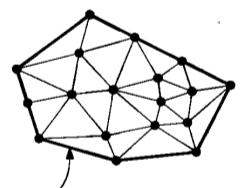
\includegraphics[width=70mm]{images/triangulacja1.png}
\caption{Przykładowa triangulacja. Źródło \cite{geometria}}
\label{triangulationexample}
\end{figure}

\emph{Triangulacją} nazywać będziemy podział $n$-wymiarowej przestrzeni na~\emph{sympleksy}~(trójkąty, czworościany). W~szczególności, dla~płaszczyzny będą to~trójkąty, stąd nazwa \emph{triangulacja}. Wszystkie trójkąty muszą łączyć~się w~całość poprzez wspólne krawędzie, lub~wspólne wierzchołki.

Niech $P:=\{ p_{1},p_{2},...,p_{n} \}$ będzie zbiorem punktów na~płaszczyźnie euklidesowej $E$. Przez \emph{maksymalny podział płaszczyzny}~$\mathcal{S}$ rozumieć będziemy taki graf o~wierzchołkach w~$P$, do~którego nie~można dodać żadnej nowej krawędzi bez~tworzenia grafu nieplanarnego. Tak~więc~$\mathcal{S}$ jest \emph{triangulacją} zbioru~$P$ na~płaszczyźnie~$E$. Podstawą dla~tego stwierdzenia jest fakt, iż~każdy wielokąt na~płaszczyźnie możemy podzielić na~trójkąty\cite{geometria}, tak więc dla~każdego pustego wielokąta w~$\mathcal{S}$ możemy dodać do~niego nowe krawędzie.

Zewnętrzne krawędzie \emph{triangulacji} zbioru punktów~$P$ zawsze tworzą jego otoczkę wypukłą. Wszystkie możliwe triangulacje zbioru~$P$ mają tę~samą ilość trójkątów i~krawędzi i~wynoszą one odpowiednio $2n-2-k$ i~$3n-3-k$, gdzie~$k$ to~ilość punktów leżących na~otoczce wypukłej.

\subsection{Wektor Kątów}

Niech~$\mathcal{T}$ będzie triangulacją~$P$ posiadającą~$m$ trójkątów. Przez~$A(\mathcal{T}) := (\alpha_{1}, \alpha_{2}, ..., \alpha_{3m})$ oznaczać będziemy posortowany rosnąco \emph{wektor~kątów} triangulacji~$\mathcal{T}$.

Mówimy, że~wektor kątów~$A(\mathcal{T'})$ jest leksykograficznie większy od~wektora kątów~$A(\mathcal{T})$, jeżeli istnieje indeks~$1 \leq i \leq 3m$ taki, że~dla~$j < i, \alpha_{j} = \alpha_{j}'$ oraz~$\alpha_{i} < \alpha_{i}'$.

Triangulację~$\mathcal{T}$ nazywamy \emph{kątowo optymalną}, jeżeli zachodzi~$A(\mathcal{T}) \geq A(\mathcal{T'})$ dla wszystkich możliwych triangulacji~$\mathcal{T'}$ zbioru~$P$. Optymalna kątowo triangulacja jest \emph{Triangulacją Delaunay}. Dodatkowo, jeżeli w~zbiorze~$P$ nie ma~czwórki punktów tworzących przyległe trójkąty i~leżących na~okręgu, to~triangulacja ta jest unikalna.

\subsection{Optymalizacja Kątów i Flip Edge}

Dla pary trójkątów~$p_{i}, p_{j}, p_{l}$ oraz~$p_{i}, p_{k}, p_{j}$ z~$\mathcal{T}$ współdzielących krawędź~$\overline{p_{i} p_{j}}$, możemy usunąć tę~krawędź i~zastąpić ją~krawędzią~$\overline{p_{k} p_{l}}$, w~wyniku czego otrzymamy triangulację~$\mathcal{T'}$. Jeżeli lokalnie dla~tej pary trójkątów minimalny kąt został zwiększony, to~nowa triangulacja~$\mathcal{T'}$ jest bardziej optymalna od~poprzedniej. Procedurę tą~nazywamy \emph{edge flip}.

\begin{figure}[ht!]
\centering
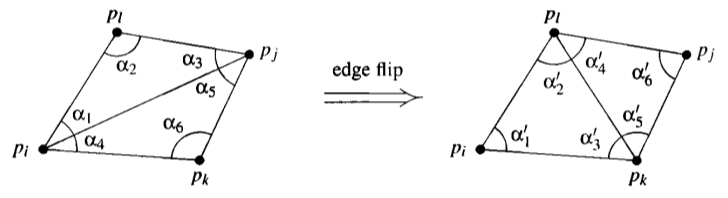
\includegraphics[width=150mm]{images/triangulacja2.png}
\caption{Zastosowanie operacji \emph{edge flip}. Źródło \cite{geometria}}
\label{edgeflip}
\end{figure}

\begin{figure}[ht!]
\centering
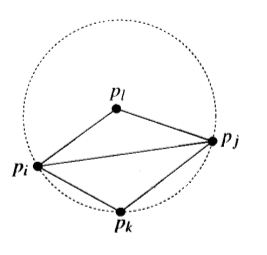
\includegraphics[width=70mm]{images/triangulacja3.png}
\caption{Okrąg opisany na trójkącie wykazujący nieoptymalną krawędź. Źródło \cite{geometria}}
\label{edgetest}
\end{figure}

Aby stwierdzić, czy dana krawędź~$\overline{p_{i} p_{j}}$ współdzielona przez trójkąty $p_{i}, p_{j}, p_{l}$ oraz $p_{i}, p_{k}, p_{j}$ z~$\mathcal{T}$ jest nieoptymalna, można to~łatwo sprawdzić poprzez narysowanie okręgu opisanego na~jednym z~tych trójkątów. Jeżeli wierzchołek drugiego trójkąta, nie~należący do~współdzielonej krawędzi, mieści się~wewnątrz tego okręgu, to~krawędź jest nieoptymalna. Jeżeli wszystkie cztery wierzchołki znajdują się na~narysowanym okręgu, to~obydwie możliwe triangulacje są~sobie równoważne.

Stosując powyższą metodę, możemy z~dowolnej triangulacji~$\mathcal{T}$ uzyskać optymalną triangulację~$\mathcal{T'}$ (nazywaną także \emph{triangulacją poprawną}) stosując poniższą procedurę.

\begin{algorithm}
\caption{$LegalTriangulation(\mathcal{T})$ \cite{geometria}}
\label{LegalTriangulation}
\begin{algorithmic}
    \WHILE{$\mathcal{T}$ contains illegal edge $\overline{p_{i} p_{j}}$}
        \STATE Let $p_{i}, p_{j}, p_{l}$ and $p_{i}, p_{k}, p_{j}$ be the two triangles adjacent to $\overline{p_{i} p_{j}}$
        \STATE Remove $\overline{p_{i} p_{j}}$ from $\mathcal{T}$, add $\overline{p_{k} p_{l}}$
    \ENDWHILE
    \RETURN $\mathcal{T}$
\end{algorithmic}
\end{algorithm}

\section{Dualność Triangulacji Delaunay i Diagramu Voronoi}

W~poprzednim rozdziale opisywaliśmy Diagram Voronoi. Podobnie jak~Triangulacja Delaunay, tworzony jest on~na podstawie zbioru punktów~$P:=\{ p_{1},p_{2},...,p_{n} \}$. Posiadając wygenerowany diagram~$Vor(P)$, tworzymy graf~$\mathcal{G}$ o~wierzchołkach w~$P$. Dla każdej krawędzi w~$Vor(P)$ rozdzielającej punkty $p_{i}, p_{j}$ dodajemy nową krawędź do~grafu~$\mathcal{G}$. Jeżeli narysujemy wszystkie krawędzie grafu~$\mathcal{G}$ jako linie proste, otrzymamy triangulację zbioru punktów~$P$. Graf ten~jest grafem dualnym dla~grafu~$Vor(P)$ -~komórki grafu~$Vor(P)$ są~wierzchołkami grafu~$\mathcal{G}$, natomiast trójkąty~$\mathcal{G}$ są~wierzchołkami w~$Vor(P)$.


\begin{figure}[ht!]
\centering
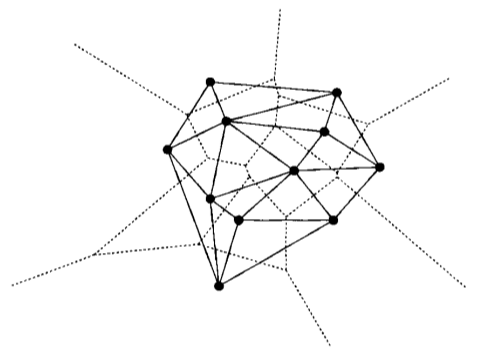
\includegraphics[width=100mm]{images/dualizm.png}
\caption{Triangulacja Delaunay i odpowiadający jej Diagram Voronoi. Źródło \cite{geometria}}
\label{duality}
\end{figure}

\section{Obliczanie Triangulacji}

Poznaliśmy już jedną metodę tworzenia Triangulacji Delaunay -~stosowanie procedury \emph{flip edge} do~momentu, w~którym nie~można zoptymalizować już~żadnej z~krawędzi. Posiada ona jednak pewne wady. Przede wszystkim operuje ona na~już~istniejącej triangulacji, więc wejście w~postaci zbioru punktów na~płaszczyźnie nie~jest~wystarczające. Dodatkowo, metoda ta~nie~jest najbardziej optymalna, gdyż jej złożoność obliczeniowa wynosi~$O(n^2)$.

\subsection{Inicjalizacja Algorytmu}

Wiemy także, że~triangulację tę~możemy uzyskać poprzez dualność Diagramu Voronoi, który także potrafimy wygenerować. Teraz rozpatrzymy algorytm generowania triangulacji wprost z użyciem losowej procedury inkrementacyjnej.

Tak jak~poprzednio, triangulację generować będziemy dla zbioru punktów~$P:=\{ p_{1},p_{2},...,p_{n} \}$. Aby uniknąć problemów z~nieograniczonymi trójkątami na~brzegach triangulacji, dodajemy do~niej zewnętrzny trójkąt $p_{-1}, p_{-2}, p_{-3}$, zawierający w~swoim wnętrzu wszystkie punkty z~$P$, jednak jego wierzchołki nie~mogą leżeć wewnątrz żadnego opisanego na~dowolnej trójce punktów z~$P$. Będziemy nazywać go \emph{supertrójkątem}. Oznacza~to, że~obliczamy triangulację nie~tylko zbioru $P$, ale $P \cup \{p_{-1}, p_{-2}, p_{-3}\}$.


\begin{figure}[ht!]
\centering
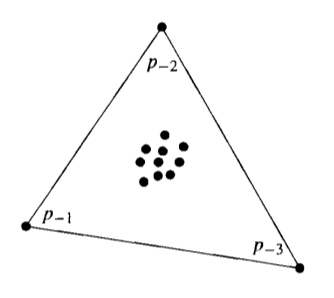
\includegraphics[width=80mm]{images/triangulacja5.png}
\caption{Przykład supertrójkąta zawierającego w sobie cały zbiór $P$. Źródło \cite{geometria}}
\label{supertriangle}
\end{figure}

Jak już~powiedzieliśmy, algorytm jest losowy i~inkrementacyjny. Oznacza~to, że~w~każdym kroku do~triangulacji dodawany jest jeden, losowo dobrany, jeszcze nie~użyty punkt~$p_{r}$ ze~zbioru~$P$. Najpierw ustalamy, w~którym trójkącie dodany zostanie nowy punkt. Metoda ustalania opisana zostanie za~chwilę. Następnie dodajemy nowe krawędzie łączące nowo dodany punkt z~wierzchołkami trójkąta, we~wnętrzu którego się~znajduje. Jeżeli punkt~$p_{r}$ wypadnie na~już istniejącej krawędzi, krawędź~ta jest najpierw usuwana, a~następnie punkt łączony jest nowymi krawędziami ze~wszystkimi wierzchołkami powstałego czworoboku.

\begin{figure}[ht!]
\centering
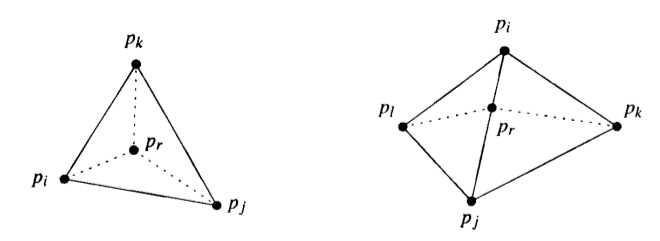
\includegraphics[width=130mm]{images/triangulacja6.png}
\caption{Możliwe przypadki umiejscowienia nowego punktu w triangulacji. Źródło \cite{geometria}}
\label{newpointposition}
\end{figure}

\subsection{Poprawianie Nieoptymalnych Krawędzi}

Ponieważ po~wykonaniu powyższych operacji uzyskana triangulacja może nie~być optymalna, w~każdym kroku bieżący zbiór punktów optymalizowany jest pod kątem maksymalizacji minimalnych kątów metodą \emph{flip edge} poprzez zastosowanie procedury $LegalizeEdge$ na~wszystkich potencjalnie nieoptymalnych krawędziach.

\begin{algorithm}
\caption{$LegalizeEdge(p_{r}, \overline{p_{i} p_{j}}, \mathcal{T})$ \cite{geometria}}
\label{LegalizeEdge}
\begin{algorithmic}
    \IF{$\overline{p_{i} p_{j}}$ is illegal}
        \STATE Let $p_{i} p_{j} p_{k}$ be a triangle adjacent to $p_{r} p_{i} p_{j}$ along $\overline{p_{i} p_{j}}$
        \STATE Replace $\overline{p_{i} p_{j}}$ with $\overline{p_{r} p_{k}}$
        \STATE $LegalizeEdge(p_{r}, \overline{p_{i} p_{k}}, \mathcal{T})$
        \STATE $LegalizeEdge(p_{r}, \overline{p_{k} p_{j}}, \mathcal{T})$
    \ENDIF
\end{algorithmic}
\end{algorithm}

\begin{algorithm}
\caption{$DelaunayTriangulation(P)$ \cite{geometria}}
\label{DelaunayTriangulation}
\begin{algorithmic}
    \STATE Initialize triangulation $\mathcal{T}$ with triangle $p_{-1} p_{-2} p_{-3}$
    \STATE Compute random permutation $p_{1}, p_{2}, ..., p_{n}$ of $P$
    \FOR{$r$ from 1 to $n$}
        \STATE Find triangle $p_{i} p_{j} p_{k} \in \mathcal{T}$ containing $p_{r}$
        \IF{$p_{r}$ lies inside triangle $p_{i} p_{j} p_{k}$}
            \STATE Add edges $\overline{p_{r} p_{i}}, \overline{p_{r} p_{j}}, \overline{p_{r} p_{k}}$ to $\mathcal{T}$
            \STATE $LegalizeEdge(p_{r}, \overline{p_{i} p_{j}}, \mathcal{T})$
            \STATE $LegalizeEdge(p_{r}, \overline{p_{j} p_{k}}, \mathcal{T})$
            \STATE $LegalizeEdge(p_{r}, \overline{p_{k} p_{i}}, \mathcal{T})$
        \ELSE
            \STATE $p_{r}$ lies on edge $\overline{p_{i} p_{j}}$
            \STATE Find $p_{l} \neq p_{k}$ forming triangle with $\overline{p_{i} p_{j}}$ in $\mathcal{T}$
            \STATE Remove $\overline{p_{i} p_{j}}$ from $\mathcal{T}$
            \STATE Add edges $\overline{p_{r} p_{i}}, \overline{p_{r} p_{j}}, \overline{p_{r} p_{k}}, \overline{p_{r} p_{l}}$ to $\mathcal{T}$
            \STATE $LegalizeEdge(p_{r}, \overline{p_{i} p_{k}}, \mathcal{T})$
            \STATE $LegalizeEdge(p_{r}, \overline{p_{j} p_{k}}, \mathcal{T})$
            \STATE $LegalizeEdge(p_{r}, \overline{p_{i} p_{l}}, \mathcal{T})$
            \STATE $LegalizeEdge(p_{r}, \overline{p_{j} p_{l}}, \mathcal{T})$
        \ENDIF
    \ENDFOR
    \STATE Discard points $p_{-1} p_{-2} p_{-3}$ and all their incident edges from $\mathcal{T}$
    \RETURN $\mathcal{T}$
\end{algorithmic}
\end{algorithm}

Ponieważ każda zamiana krawędzi może spowodować, że w~przylegających do~niej trójkątach mogą pojawić~się nowe nieprawidłowe krawędzie, procedura wywołuje~się rekursywnie. Ponieważ każde wykonanie tej operacji powiększa wektor kątów, nie~ma ryzyka, że~operacja będzie cyklicznie wywoływać~się w~nieskończoność.

Do~omówienia pozostały dwie istotne części algorytmu. Są~nimi: wybór trójkąta, w~którym znajduje~się~$p_{r}$ oraz testowanie poprawności krawędzi w~trójkątach zawierających jeden z~wierzchołków supertrójkąta.

\subsection{Wyszukiwanie Trójkątów}

Wyszukiwanie trójkątów zrealizujemy poprzez użycie skierowanego, niecyklicznego grafu~$\mathcal{D}$. Jego liście oznaczać będą trójkąty bieżącej triangulacji~$\mathcal{T}$, wewnętrzne wierzchołki będą symbolizować trójkąty, które istniały w~triangulacji we~wcześniejszych krokach, lecz zostały już~zastąpione. Graf~$\mathcal{D}$ inicjowany~jest pojedyńczym węzłem-liściem odpowiadającym supertrójkątowi~$p_{-1} p_{-2} p_{-3}$.

Aby podzielić trójkąt~$p_{i} p_{j} p_{k}$ na~trzy (lub~dwa) nowe trójkąty, dodajemy do~jego liścia nowe liście odpowiadające jego podziałowi, zamieniając go~w~wierzchołek wewnętrzny. Jeżeli zamieniamy dwa trójkąty~$p_{k} p_{i} p_{j}$ i~$p_{i} p_{j} p_{l}$ na~trójkąty~$p_{k} p_{i} p_{l}$ i~$p_{k} p_{l} p_{j}$ przez operację \emph{edge~flip}, tworzymy dla nich dwa nowe liście i~podłączamy do~węzłów~$p_{k} p_{i} p_{j}$ i~$p_{i} p_{j} p_{l}$. Używając tak utworzonego grafu~$\mathcal{D}$ do~zlokalizowania~$p_{r}$ aby dodać do~triangulacji, zaczynamy od~węzłą supertrójkąta i~sprawdzamy, w~którym z~jego dzieci mieści~się nowy punkt. Powtarzamy tę~operację aż~dotrzemy do~jednego z~liści.

\subsection{Nieprawidłowe Krawędzie Brzegowe}

Ostatnią kwestią jest wykrywanie nieprawidłowych krawędzi w~trójkątach zawierających punkty~$p_{-1}, p_{-2}$, lub~$p_{-3}$. Zaczniemy od określenia koordynatów tych punktów tak, aby zawierał~się w~nim cały zbiór~$P$. Niech~$M$ będzie największą wartością bezwzględną ze~wszystkich koordynatów punktów z~$P$. Wybieramy punkty $p_{-1} := (3M, 0)$, $p_{-2} := (0, 3M)$ oraz $p_{-3} := (-3M, -3M)$.

Przy sprawdzaniu krawędzi, traktujemy punkt~$p_{-1}$ jako leżący na~zewnątrz okręgu opisanego na~dowolnej trójce punktów z~$P$, $p_{-2}$ jako leżący na~zewnątrz okręgu opisanego na~dowolnej trójce punktów z~$P \cup \{p_{-1}\}$, $p_{-3}$ jako leżący na~zewnątrz okręgu opisanego na~dowolnej trójce punktów z~$P \cup \{p_{-1}, p_{-2}\}$. Sprawdzając krawędź $\overline{p_{i} p_{j}}$ oraz punktów $p_{k}, p_{l}$ tworzących razem z nią dwa trójkąty stosujemy następujące warunki:
\begin{itemize}
\item
jeżeli $i,j < 0$ to krawędź jest prawidłowa
\item
jeżeli $i, j, k, l > 0$ to postępujemy standardowo
\item
dokładnie jeden z~indeksów~$i, j, k, l$ jest negatywny, to~jeżeli jest~to~$i$ lub~$j$, krawędz jest nieprawidłowa, w~innym przypadku pozostawiamy ją~niezmienioną
\item
dokładnie dwa z~indeksów~$i, j, k, l$ są~negatywne, to~jeden indeks z~pary~$i, j$ oraz jeden z~pary~$k, l$ są~negatywne (przypadek negatywnej pary~$i, j$ obsłużyliśmy powyżej), jeżeli negatywny indeks z~$i, j$ jest mniejszy od~negatywnego indeksu z~$k, l$, to~krawędź jest prawidłowa, w~przeciwnym wypadku zmieniamy~ją
\item
dokładnie trzy z~indeksów~$i, j, k, l$ są~negatywne, ten przypadek nie może wystąpić
\end{itemize}

\chapter{Przejście z Przestrzeni 2D do 3D}

Poznaliśmy już właściwości i~metody tworzenia \emph{Triangulacji Delaunay} oraz \emph{Diagramu Voronoi}. Do~tej pory zajmowaliśmy~się jednak jedynie przypadkami dwuwymiarowymi. Obydwa zagadnienia mogą być jednak rozpatrywane w~przestrzeni $n$-wymiarowej. W~tym rozdziale omówimy istotne różnice pomiędzy przypadkami dwu-~i~trójwymiarowymi.

\section{Triangulacja Delaunay}

\subsection{Właściwości}

Do~tej pory rozważaliśmy podział płaszczyzny na~trójkąty, jednak w~przypadku przestrzeni używać będziemy czworościanów. Czworościany te~nadal zbudowane~są z~trójkątów, jednak triangulacja składa~się z~kompletnych brył i~nie~może w~niej wystąpić czworościan, w~którym brakuje jednej ze~ścian.

Triangulacja zdefiniowana jest dla przestrzeni $n$-wymiarowej, możemy więc spodziewać~się, że~jej właściwości zarówno w~2D jak~i~w~3D będą takie same. W rzeczywistości tak jest, chociaż niektóre właściwości opisane dla przestrzeni dwuwymiarowej nie mogą być przeniesione wprost do przestrzeni trójwymiarowej i muszą być zinterpretowane w nieco inny sposób.

W poprzednim rozdziale przedstawiliśmy triangulację, jako podział płaszczyzny na sympleksy współdzielące wierzchołki i~krawędzie. Tą~samą definicję możemy zastosować w~3D, stosując jako sympleks czworościan oraz dodając do~niej współdzielenie ścian. Wiedzieliśmy, że~składa~się ona jedynie z~sympleksów, ponieważ dowolny wielokąt można podzielić na~trójkąty. Zasada ta~obowiązuje także w~przypadku brył wypukłych, teraz jednak zamiast pojedyńczych krawędzi, dodajemy trójkątne ściany (co~może sprowadzać~się do~dodania kilku, jednej, lub żadnych nowych krawędzi), aż~do~momentu, w~którym dodanie kolejnej spowoduje stworzenie grafu nieplanarnego. Jak się~jednak okazuje, możemy uzyskać poprawną triangulację nie~wypełniając jej całkowicie możliwymi krawędziami. Jeżeli nasz graf używa już wszystkich punktów~$P$, zawiera tylko kompletne czworościany i~tworzy bryłę wypukłą, to~możemy zakończyć jego tworzenie.

Jako przykład weźmy dwa czworościany~$A B C D$ oraz~$A B C E$ współdzielące ścianę~$A B C$. Jeżeli odległość pomiędzy punktami~$D$ i~$E$ jest na~tyle mała, że~wewnątrz kuli, której średnicą jest~ta krawędź nie~zawiera~się żaden z~punktów~$A, B, C$, to~dodanie krawędzi~$\overline{D E}$ da~nam optymalniejszą triangulację. Jeżeli jednak wewnątrz (lecz~nie~na~powierzchni) wspomnianej kuli znajduje się inny punkt, to~lepiej jest nie~dodawać nowej krawędzi. W~obydwu przypadkach, niezależnie od~dodania krawędzi $\overline{D E}$, mamy poprawne triangulacje (w~rozumieniu ogólnym).

Nasz graf musi być planarny, co~w~przypadku~2D oznaczało, że~żadna para krawędzi nie może~się przecinać. Jednak w~przypadku trójwymiarowym to~nie~wystarczy. Spójrzmy na~ten problem poprzez elementy podziału naszej przestrzeni - sympleksy. Poprzednio używaliśmy trójkątów zbudowanych z~krawędzi, które nie~mogły się~przecinać. Teraz używamy czworościanów zbudowanych z~trójkątów, więc jako zasadę planarności możemy przyjąć, że~te~trójkąty nie~mogą się~przecinać. Trójkąt~$A$ przecina trójkąt~$B$ w~przestrzeni trójwymiarowej, jeżeli którakolwiek z~krawędzi trójkąta~$A$ przecina którąkolwiek z~krawędzi trójkąta $B$, lub krawędź z~$A$ przecina płaszczyznę trójkąta $B$, a~punkt przecięcia znajduje się~we~wnętrzu trójkąta~$B$. Tak więc nasza poprzednia definicja planarności musi zostać rozszerzona o~zapis, że~żadna para trójkątów w~triangulacji nie może~się przecinać. Rysunek \ref{triangulation3d} obrazuje dwa przypadki czworościanów współdzielących ścianę (oznaczoną~na~szaro), w~których dodanie krawędzi łączącej nie jest wymagane do utworzenia triangulacji, lecz jej dodanie tworzy nową, poprawną triangulację. Drugi przykład wymaga dodania jej aby zoptymalizować kąty.

\begin{figure}[ht!]
\centering
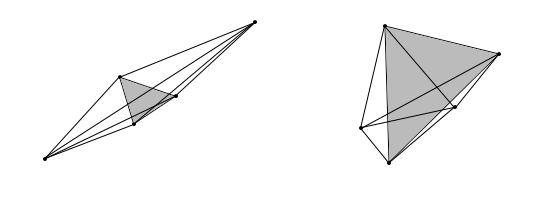
\includegraphics[width=150mm]{images/triangulacja_3d.png}
\caption{Przykład niejednoznaczności triangulacji w trzech wymiarach}
\label{triangulation3d}
\end{figure}

Jak pamiętamy, \emph{Triangulacja Delaunay} ma~na~celu maksymalizację minimalnych kątów. Jednak w~przypadku czworościanów stosować będziemy bardziej ogólną zasadę przeznaczoną dla~$n$-wymiarowych triangulacji. Zasada ta mówi, że~dla~każdego czworościanu triangulacji, sfera opisana na~tym czworościanie nie może zawierać żadnego innego punktu z~tej~triangulacji.

\subsection{Obliczanie}

W~poprzednim rozdziale opisaliśmy optymalny sposób wyliczania \emph{Triangulacji Delaunay} dla przypadku dwuwymiarowego. Niestety, w~trzech wymiarach metoda ta~nie~zadziała, ponieważ wykonanie operacji \emph{flip edge} nie jest możliwe - ściana dzieląca może być zamieniona na inną w~dwóch różnych płaszczyznach, lub też dwa czworościany muszą zostać zamienione na~trzy inne. Z~tego powodu do~obliczania triangulacji używać będziemy algorytmu Bowyera-Watsona. Podobnie jak poprzednio, jest to~algorytm inkrementacyjny i~losowy. Jest on~bardziej złożony obliczeniowo, można go~jednak stosować w~dowolnej, $n$-wymiarowej przestrzeni.

Tak jak poprzednio, obliczenia zaczynamy od~dodania supersympleksu zawierającego w sobie wszystkie punkty ze~zbioru~$P$. W~przypadku trójwymiarowym jest to~czworościan. Następnie w~każdym kroku algorytmu, do bieżącej triangulacji dodajemy jeden, losowo wybrany punkt $p_{r} \in P$. Aby zbudować poprawną triangulację, wyszukujemy wszystkie czworościany, dla których punkt~$p_{r}$ zawiera się w~kuli opisanej na~tym czworościanie. Każdy z~dopasowanych czworościanów jest usuwany z~triangulacji, a~jego ściany dodawane są~do~zbioru~$\mathcal{W}$. Jeżeli dana ściana znajduje się już w~tym zbiorze, to~zamiast dodawać, jest ona z~niego usuwana. W~ten sposób tworzymy pustą przestrzeń wewnątrz triangulacji zawierającą punkt $p_{r}$. Musimy teraz dodać do niej nowe czworościany, po jednym na~każdą ścianę znajdującą się w~$\mathcal{W}$, łącząc je z nowo dodanym punktem.

Wadą tego algorytmu jest~to, że~nie traktuje on~dodatkowych wierzchołków supersympleksu w~specjalny sposób, przez co~zewnętrzne krawędzie właściwej triangulacji mogą układać się~nieprawidłowo. Aby to~naprawić, należy usunąć te~wierzchołki oraz przyległe do~nich krawędzie. Potem musimy wyszukać otwarte czworościany i~dodać do~nich brakujące fragmenty.

\section{Diagram Voronoi}

\subsection{Właściwości}

Podobnie jak w~przypadku triangulacji, \emph{Diagram Voronoi} może być zastosowany w~$n$-wymiarowej przestrzeni. Dla przypadku trójwymiarowego nie ma większych różnic, poza oczywistym dodaniem kolejnego wymiaru. Zbiory najbliższych punktów dla każdego z~centrów ze~zbioru~$P$ utworzą bryły wypukłe, których ściany zbudowane są~z~wielokątów. Przedstawić je~można jako część współną zbioru półprzestrzeni ograniczonych płaszczyznami.

\subsection{Obliczanie}

Wraz z~dodaniem trzeciego wymiaru znany nam algorytm Fortune nadal działa, jednak ze~względu na~potrzebę śledzenia plaży zbudowanej z~paraboloid zamiast parabol wykrywanie odpowiednich zdarzeń komplikuje się. Kolejnym problemem jest śledzenie nie tylko rysowanych linii, ale także trójkątów. Z~tego powodu na potrzeby tej pracy zastosujemy prostszą metodę, a~mianowicie wspomniane wcześniej przecięcie półprzestrzeni.

Potencjalnym problemem przy tym podejściu jest możliwość utworzenia nieograniczonych komórek, dlatego jako bazy użyjemy prostopadłościanu obejmującego wystarczająco dużą przestrzeń. Tak przygotowaną figurę będziemy przecinać z~półprzestrzeniami tworząc pojedyńczą komórkę diagramu. Operację tę~powtarzamy dla każdego z~punktów ze~zbioru~$P$.

\chapter{Implementacja i Wyniki}

W~niniejszym rozdziale omówimy praktyczną implementację \emph{Triangulacji Delaunay} oraz \emph{Diagramu Voronoi}. Następnie pokażemy jak zastosować je~w~praktyce do~podziału bryły definiowanej poprzez siatkę wielokątów na części.

\begin{figure}[ht!]
\centering
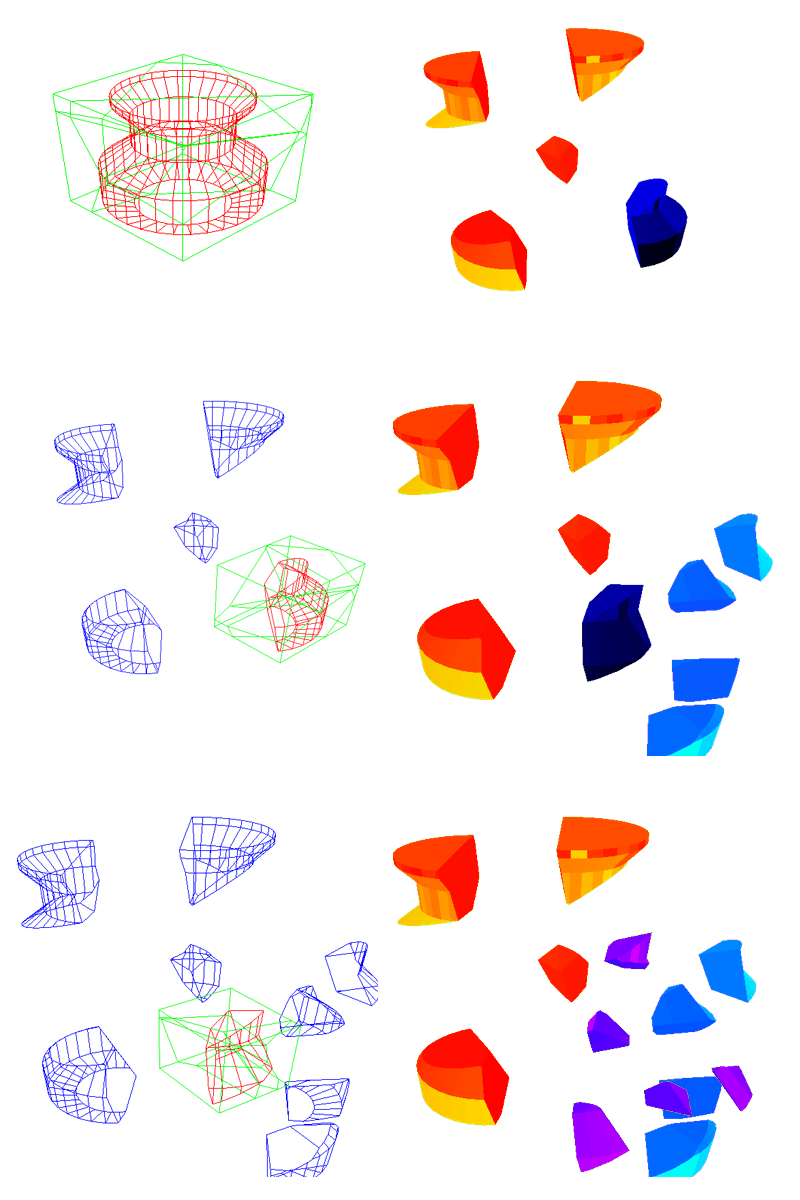
\includegraphics[width=140mm]{images/app4_1.png}
\caption{Przykład trzypoziomowego podziału obiektu}
\label{appdivisionlevels}
\end{figure}

\section{Wstępna Specyfikacja}

Przykładowa implementacja dołączona do~tej pracy napisana została w~języku~C++. Do wizualizacji użyta została biblioteki OpenGL oraz wspomagającą jej użycie GLU. Aby zapewnić interfejs użytkownika dla kontekstu OpenGL osadziliśmy go~w~oknie stworzonym z~użyciem biblioteki~QT w~wersji~4. Sama implementacja algorytmów także korzysta z~podstawowych struktur danych udostępnianych przez QT, takich, jak listy, zaawansowane łańcuchy znakowe i~obsługa wejścia plików.

\subsection{Format Wejściowy}

Jako format wejściowy aplikacja przyjmuje pliki w~standardzie OBJ, który dostępny jest w~darmowym narzędziu do~modelowania 3D o~nazwie \emph{Blender}. Korzystając z~możliwości obsługi wejścia z~pliku i~obróbki ciągów znaków udostępnianych przez środowisko~QT, stworzony został prosty parser dla wspomnianego formatu. Nie jest on~jednak pełny i~obejmuje jedynie najważniejsze aspekty potrzebne do~obróbki bryły, czyli listy wierzchołków oraz ścian. Format pozwala na~zapisanie w~pliku danych o~wektorach normalnych dla wierzchołków i ścian, teksturowaniu, oraz innych. Są one jednak ignorowane.

\subsection{Modularność Aplikacji}

Kod odpowiedzialny za~logikę obliczeń stworzony został jako część samodzielna, wymagająca jedynie biblioteki QT. Komunikuje się ona z~częścią renderującą obraz poprzez publiczny interfejs, co~pozwala na~swobodną wymianę modułu wizualizacji, oraz na~osadzenie go~wewnątrz większej aplikacji.

Przykładowy renderer pozwala na~podgląd wygenerowanych struktur:
\begin{itemize}
\item
trianulacji zbioru punktów~$P$ lub samego supersympleksu
\item
komórek diagramu dzielących przestrzeń dookoła obiektu z~możliwością wyświetlania wybranej komórki
\item
fragmentów obiektu po podziale z~możliwością wyświetlania wybranego fragmentu
\end{itemize}

Aby pozwolić na~wierniejsze odwzorowanie podziału obiektu, aplikacja pozwala na~wykonanie wszystkich operacji na~każdym z wygenerowanych fragmentów, zapewniając nam możliwość hierarchicznego podziału.

Zastosowane algorytmy pozwalają na~całkowicie poprawne podziały jedynie dla obiektów wypukłych. W~przypadku niewielkich wklęśnięć aplikacja prawdopodobnie zachowa się poprawnie, nie można tego jednak zagwarantować.

\section{Obliczanie Triangulacji}

W~celu obliczenia triangulacji punktów podziału naszego obiektu, aplikacja korzysta z~algorytmu Bowyera-Watsona opisanego w poprzednim rozdziale.

\begin{figure}[ht!]
\centering
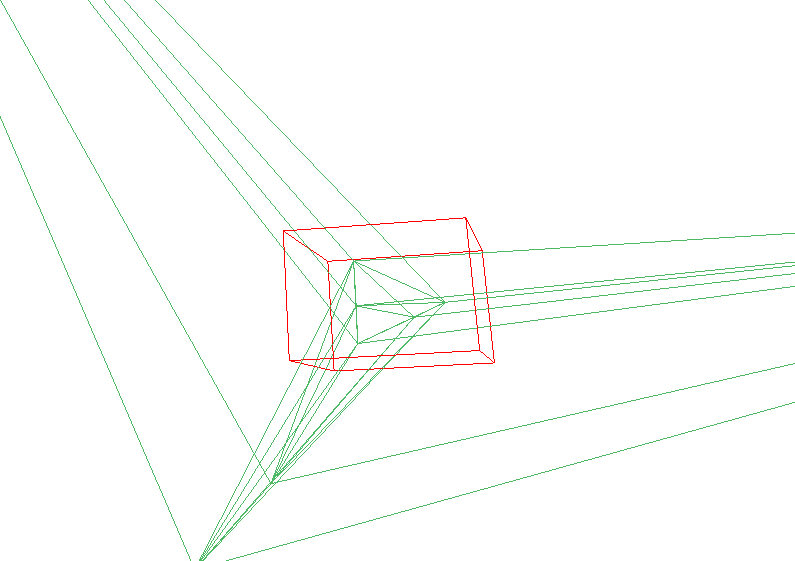
\includegraphics[width=140mm]{images/app1_1.png}
\caption{Triangulacja wygenerowana przez aplikację}
\label{apptriangulation}
\end{figure}

\subsection{Struktury Danych}

Podstawową strukturą danych dla naszego algorytmu jest lista obiektów \code{Tetrahedron}. Obiekty tej klasy przechowują informację o~tym, które z~punktów podziału stanowią wierzchołki czworościanu. Korzystając z~tej informacji obliczana jest pozycja punktu stanowiącego środek sfery opisanej na~tym czworościanie, oraz kwadrat jego odległości od~wierzchołków. Obydwie z~tych właściwości są~dla danego czworościanu niezmienne, możemy więc obliczyć je~raz i~przechowywać wyniki do~wykorzystania w~wyszukiwaniu sympleksów obejmujących nowo dodane punkty.

Podczas dodawania nowego punktu, każdy z~czworościanów mający go~w~zasięgu musi zostać usunięty z~triangulacji. Aby śledzić które z~ich ścian muszą zostać użyte do~zbudowania nowych sympleksów, tworzymy listę przechowującą dla każdej ze~ścian ilość używających ją~czworościanów. Jak łatwo się domyślić, wszystkie wpisy mogą zawierać jedynie wartości od~0 do~2. Za~każdym razem, gdy usuwany jest jeden z~czworościanów, licznik użyć dla każdej jest dekrementowany, po~czym ściana dodawana jest do~listy ścian potencjalnie tworzących nowe struktury.

Kolejna pętla sprawdza wszystkie ściany zebrane w kroku poprzednim pod kątem ich użycia.
\begin{itemize}
\item
jeżeli ściana posiada ilość użyć równą~1 oznacza~to, że~oddziela ona istniejący czworościan od~pustej przestrzeni stworzonej dookoła nowego punktu i~należy użyć jej do~stworzenia nowego czworościanu
\item
jeżeli ściana posiada ilość użyć równą~0 oznacza~to, że ściana ta~rozdzielała dwa sąsiadujące ze~sobą czworościany mające w~swoim zasięgu nowy punkt i~należy ją~pominąć
\item
ściana posiadająca ilość użyć równą~2 nigdy nie powinna się tu~pojawić, gdyż jedna ściana może być użyta przez conajwyżej dwa czworościany
\end{itemize}

Dodatkowo, w~czasie budowania nowych czworościanów sprawdzamy, czy nowo dodawane ściany nie zostały już utworzone poprzednio i~używamy ich ponownie.

\section{Obliczanie Diagramu}

Obliczanie \emph{Diagramu Voronoi} zrealizowane zostało z~użyciem metody opisanej w~rozdziale czwartym. Powodem tego jest o~wiele prostsza implementacja względem algorytmu Fortune dla trzech wymiarów. Niektóre ze szczegółów implementacyjnych pochodzą z~zasobów W:BLUT \cite{fvan}.

\begin{figure}[ht!]
\centering
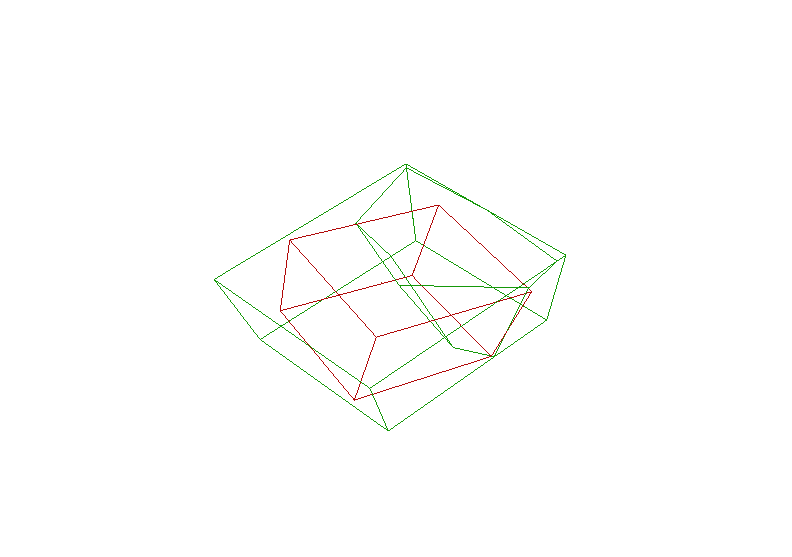
\includegraphics[width=140mm]{images/app2_1.png}
\caption{Komórka Voronoi obliczona przez aplikację}
\label{appcell}
\end{figure}

\subsection{Struktury Danych}

Jak wspomniano wcześniej, potrzebna jest nam bazowa bryła, od~której możemy zacząć tworzenie komórek. W~przykładowej aplikacji użyty w~tym celu został prostopadłościan zawierający w~swoim wnętrzu dzielony obiekt. Podczas wczytywania jego wierzchołków wybierane są~ekstremalne wartości dla każdego z~wymiarów, po~czym na~ich podstawie tworzone jest wspomniany prostopadłościan.

Diagram przechowywany jest w~postaci listy obiektów \code{VoronoiCell}, zawierających następujące informacje:
\begin{itemize}
\item
lista wierzchołków budowanej komórki; na początku zawiera ona wszystkie wierzchołki bazowej bryły, przy każdym cięciu dodawane są~punkty przecięcia krawędzi z~płaszczyzną oraz usuwane punkty odcięte
\item
lista półkrawędzi, każda z nich zawiera wskaźniki na punkt początkowy, krawędź, ścianę oraz półkrawędzie: następującą oraz odwrotną, tworząc w~ten sposób zamknięte łańcuchy
\item
lista krawędzi, każda składa się z pary przeciwnych półkrawędzi
\item
lista ścian, każda z~nich posiada wskaźnik na~półkrawędź będącą początkiem tworzącej ją~łańcucha, oraz opcjonalnie wskaźnik na~obiekt płaszczyzny użytej do~utworzenia danej ściany
\end{itemize}

\subsection{Przebieg Algorytmu}

W~każdym kroku algorytmu wybierany jest jedno z~centrów ze~zbioru~$P$, po~czym następuje iteracja po~pozostałych punktach z~tego zbioru. Dla każdej pary obliczane jest równanie płaszczyzny przecinającej odcinek je~łączący pod kątem prostym i~znajdujący się na~jego środku.

Płaszczyzna ta~użyta zostaje do~przecięcia bieżącej siatki komórki. Część znajdująca się po stronie centrum zostaje zachowana, pozostała jest odrzucana. Przeciętą siatkę przechowujemy w tymczasowych strukturach danych, których zawartość przepisaywana jest do obiektu komórki po zakończeniu bieżącego cięcia. Zanim jednak dokonywane jest przecięcie, sprawdzane zostają dwa istotne warunki: jeżeli cała bryła znajduje się~po~stronie centrum, jej struktura nie jest zmieniana, jeżeli natomiast cała bryła znajduje się za~płaszczyzną tnącą, zamiast cięcia jest ona odrzucana w~całości. Kryterium to~sprawdzane jest poprzez określenie strony, po~której znajdują się wszystkie wierzchołki bryły.

Kiedy stwierdzimy, że~potrzebne jest cięcie, wykonywane jest kilka operacji. Pierwszą z~nich jest wyszukanie krawędzi przecinających płaszczyznę i~zapisanie ich w~tymczasowej tablicy. Drugą jest dokonanie cięcia poszczególnych ścian bieżącej siatki. Następnie wykonane zostaje dodanie nowej ściany na~płaszczyźnie tnącej. Cięcie kończy się na~przepisaniu zawartości struktur (wierzchołków, półkrawędzi, krawędzi i~ścian) tymczasowych do~obiektu komórki.

Wyszukanie przeciętych krawędzi jest trywialne i~sprowadza się do przejrzenia listy krawędzi i~sprawdzenia, czy ich wierzchołki leżą po przeciwnych stronach płaszczyzny.

\subsection{Cięcie Ścian}

Operację przecięcia ściany rozpoczynamy podobnie do~przecięcia całej figury, czyli od~sprawdzenia, czy cała ściana nie leży przed lub za~płaszczyzną tnącą. W~takim przypadku odpowiednio zachowujemy lub odrzucamy całą ścianę. Jeżeli jednak potrzebne jest cięcie, tworzymy nową, tymczasową ścianę, która narazie jest pusta. Zaczynając od~półkrawędzi, na~którą wskazuje oryginalna ściana iterujemy po~łańcuchu. Do zapamiętania po~której stronie płaszczyzny jesteśmy używamy flagi \code{side}, którą inicjujemy poprzez sprawdzenie po~której stronie płaszczyzny znajduje się wierzchołek pierwszej półkrawędzi.

Iterując po~łańcuchu półkrawędzi, jeżeli flaga \code{side} zawiera wartość \code{true}, przepisujemy bierzącą półkrawędź do~tymczasowej ściany. W~przeciwnym wypadku, półkrawędź jest pomijana. Następnie, niezależnie od stanu flagi, sprawdzamy, czy bieżąca półkrawędź jest przecięta przez płaszczyznę. Jeżeli tak, to~do~tymczasowej ściany dodajemy dodatkową krawędź oraz odwracamy wartość flagi. Wierzchołkiem dla dodatkowej krawędzi jest punkt przecięcia krawędzi oryginalnej ściany oraz płaszczyzny. Punkt ten dodawany jest do~listy \code{newFaceVertices}.

Aby zbudować poprawny łańcuch, w~zmiennej \code{lastCreatedEdge} przechowujemy ostatnio dodaną półkrawędź. Kiedy dodawana jest nowa półkrawędź, łączymy ją~z~przechowywaną w zmiennej, po~czym ustawiamy wartość zmiennej na~dodaną półkrawędź.

Wskaźnik na~pierwszą dodaną półkrawędź dodany zostaje do~tymczasowej ściany. Jeżeli oryginalna ściana posiadała wskaźnik na~płaszczyznę, jest on~kopiowany do~nowej struktury. Kiedy iteracja ponownie dotrze do~pierwszej półkrawędzi oryginalnej ściany, łańcuch jest zamykany i~operacja przecięcia kończy się.

W~algorytmie określamy punkty jako znajdujące się \emph{przed} lub \emph{za} płaszczyzną. Punkt znajdujący się \emph{przed} oznacza, że~dla płaszczyzny~$P$ określonej przez punkt~$V$ oraz wektor normalny~$N$, punkt ten znajduje się po~stronie wskazywanej przez zwrot wektora normalnego.

\begin{algorithm}
\caption{$CutFace(F, P)$}
\label{CutFace}
\begin{algorithmic}
    \IF{whole face $F$ in front of plane $P$}
        \RETURN F
    \ENDIF
    \IF{whole face $F$ in behind plane $P$}
        \RETURN NULL
    \ENDIF
    \STATE \code{currentHalfEdge := F->halfEdge}
    \STATE side := (is \code{currentHalfEdge->vertex} in front of $P$)
    \STATE Create new face $F'$
    \REPEAT
        \IF{\code{side == true}}
            \STATE Copy \code{currentHalfEdge} into $F'$
        \ENDIF
        \IF{\code{currentHalfEdge} is split edge}
            \STATE Retrieve split vertex $V$
            \STATE Create \code{VoronoiHalfEdge} using $V$ and add to $F'$
            \STATE \code{side := !side}
        \ENDIF
        \STATE \code{currentHalfEdge := currentHalfEdge->next}
    \UNTIL{\code{currentHalfEdge == F->halfEdge}}
    \RETURN $F'$
\end{algorithmic}
\end{algorithm}

\subsection{Tworzenie Nowej Ściany}

Do omówienia pozostała operacja stworzenia nowej ściany znajdującej się~na~płaszczyźnie tnącej. Służy do~tego wspomniana wcześniej lista wierzchołków \code{newFaceVertices}. Najpierw jednak należy dokonać parowania półkrawędzi znajdujących się na~tymczasowej liście. Przeglądając listę, dla każdej krawędzi zaczynającej się~w~punkcie~$A$, wskazującej na~półkrawędź o~wierzchołku~$B$ i~nie posiadającą jeszcze pary, wyszukujemy w~tej samej liście półkrawędzi o~wierzchołku~$B$ i~wskazującą na~półkrawędź o~wierzchołku~$A$. Łączymy te~półkrawędzie tworząc kompletną krawędź.

Gdy wszystkie możliwe półkrawędzie zostały już sparowane, przechodzimy do właściwego tworzenia ściany. Dodajemy nowy obiekt \code{VoronoiFace} do~listy tymczasowej, a~następnie tworzymy nowe półkrawędzie korzystając z~wierzchołków \code{newFaceVertices} dodając je~do~listy \code{newHalfEdges}. Każda z~nich należy do~nowej ściany, nie są~one jednak połączone w~zamknięty łańcuch. Aby tego dokonać skorzystamy z~faktu, że wszystkie ściany przyległe do~nowej składają się z~kompletnych łańcuchów, oraz z~tego, że~wszystkie możliwe krawędzie zostały sparowane.

Najpierw musimy sparować luźne krawędzie. Aby tego dokonać, dla każdej każdej z~półkrawędzi z~\code{newHalfEdges} zaczynającej się w~punkcie~$A$, wyszukujemy półkrawędź znajdującą się w~jednej z~pozostałych ścian, która zaczyna się~w~punkcie~$B$, wskazuje na~półkrawędź zaczepioną w~punkcie~$A$, oraz nie posiadającą jeszcze swojej pary.

Możemy teraz przejść do~łączenia półkrawędzi z~\code{newHalfEdges} w~zamknięty łańcuch. Dla każdej z~nich, wyszukujemy następnik poprzez sąsiadujące ściany przechodząc wskaźniki w kolejności \code{newHalfEdge->pair->next->pair->next->pair}.

\begin{figure}[ht!]
\centering
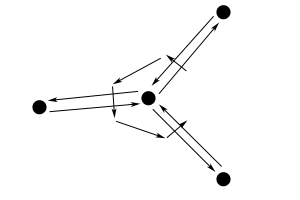
\includegraphics[width=100mm]{images/chain.png}
\caption{Ilustracja wyboru półkrawędzi do połączenia w łańcuch}
\label{chain}
\end{figure}

Teraz pozostaje nam tylko przypisanie płaszczyzny tnącej do~właśnie utworzonej ściany, kończąc w~ten sposób cięcie bierzącej siatki.

\begin{algorithm}
\caption{$BuildCutFace(V, P)$}
\label{BuildCutFace}
\begin{algorithmic}
    \STATE Create new face $F'$
    \STATE Create new list \code{newHalfEdges}
    \FOR{\code{vertex} in list V}
        \STATE Create new \code{cutHalfEdge} using \code{vertex}
        \STATE Add \code{cutHalfEdge} to list \code{newHalfEdges}
        \FOR{\code{halfEdge} in list \code{allHalfEdges}}
            \IF{halfEdge->next->v == vertex}
                \STATE Pair \code{halfEdge} and \code{cutHalfEdge}
                \STATE Break loop
            \ENDIF
        \ENDFOR
    \ENDFOR
    \FOR{\code{cutHalfEdge} in \code{newHalfEdges}}
        \STATE \code{cutHalfEdge->pair->next->pair->next->pair->next := cutHalfEdge}
    \ENDFOR
    \STATE \code{$F'$->p = P}
    \RETURN $F'$
\end{algorithmic}
\end{algorithm}

\section{Podział Bryły}

Skoro wiemy już jak podzielić prostopadłościan na~poszczególne komórki \emph{Diagramu Voronoi}, podzielenie wczytanego obiektu na~fragmenty jest łatwe. Korzystając z~już wygenerowanych komórek, powtarzamy tą~samą procedurę co~poprzednio, tym razem jednak jako bazowej bryły używamy wczytanego obiektu. Aby nie wykonywać dużej ilości nadmiarowych cięć, zamiast dwa razy iterować po~punktach ze~zbioru centrów, tym razem iterujemy po~wygenerowanych komórkach i~ich ścianach.

\begin{figure}[ht!]
\centering
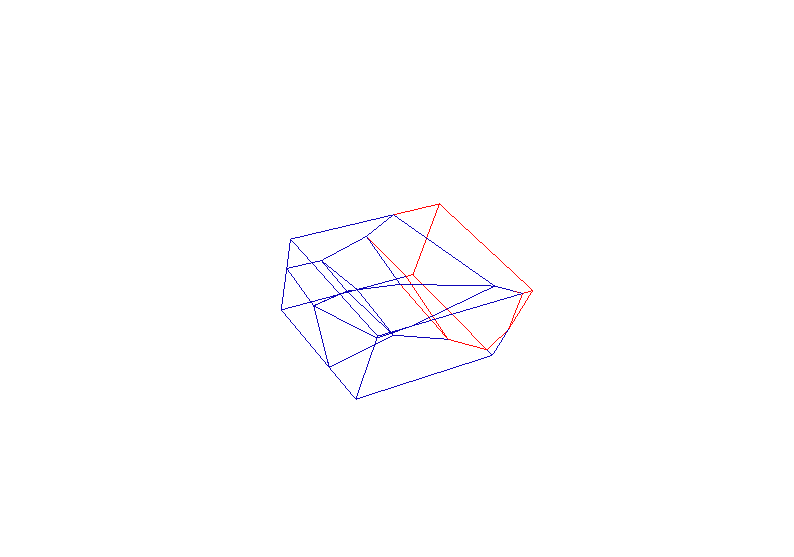
\includegraphics[width=140mm]{images/app3_1.png}
\caption{Bryła podzielona w aplikacji na pięć fragmentów}
\label{newpointposition}
\end{figure}

Dla każdej komórki diagramu rozpoczynamy od~nowej kopii bryły, wybierając płaszczyzny ze~ścian tej komórki i~wykonując takie same cięcia, jak omówione powyżej. Należy zauważyć, że~nie wszystkie ze~ścian komórek diagramu będą posiadać płaszczyzny tnące. Mowa tu~o~oryginalnych ścianach prostopadłościanu wyjściowego z~poprzedniego kroku. Ponieważ cięcie z~użyciem ich płaszczyzn byłoby bezcelowe, są~one pomijane.

Po~zakończeniu procedury otrzymujemy strukturę podobną do~tej z~kroku poprzedniego, tym razem jednak zawartą jedynie w~dzielonym obiekcie. Ostatnim krokiem programu jest wygenerowanie z~listy obiektów typu \code{VoronoiCell} nowych obiektów klasy \code{SolidObject}, dzięki czemu będziemy mogli traktować je indywidualnie i~kontynuować na~nich podziały.

\chapter{Dalsza Praca}

W~ostatnim rozdziale przedstawione zostaną możliwe ulepszenia projektu dołączonego do~tej pracy, a~także potencjalne dalsze ścieżki rozwoju przedstawionego tematu.

\section{Optymalizacja przykładowej implementacji}

Jak nietrudno zauważyć, przedstawiona w~poprzednim rozdziale implementacja podziału z~użyciem diagramu Voronoi daleka jest od~optymalnej. Przede wszystkim triangulacja nie jest potem wykorzystywana w~samym diagramie, tak więc jej obliczenie jest tylko zbędnym balastem. Patrząc jednak na~sposób generowania komórek diagramu można znaleźć dla niej zastosowanie. Jeżeli wykorzystamy informacje o~najbliższych punktach dla każdego z~centrów zawarte w~triangulacji, możemy wyeliminować cięcia, które nie mają wpływu na ostateczny kształt komórki diagramu, przez co są całkowicie zbędne.

Pośredni diagram dzielący przestrzeń dookoła obiektu także nie jest niezbędny i~istnieje on~jedynie w~celach prezentacyjnych. Pozwala to~zwizualizować kolejne etapy podziału bryły, jednak z~punktu widzenia ostatecznego wyniku może zostać pominięte.

Sama implementacja także może zostać zoptymalizowana pod kątem zużycia pamięci oraz czasu procesora. Testowana była ona na maszynie posiadającej dwurdzeniowy procesor taktowany zegarem 1,2GHz, 2GB pamięci ram oraz układ graficzny wspierający standard OpenGL w~wersji 1.3. Aby móc generować podziały w~czasie rzeczywistym, nie można użyć więcej niż 10 centrów w~jednym podziale, co~w~praktycznych zastosowaniach może nie być wystarczające.

Warto także zauważyć, że~podczas obliczania samego diagramu, operacje dla każdego z~centrów są~całkowicie niezależne. Jest to~bardzo dobra okazja do~zrównoleglenia działania programu poprzez zastosowanie technologii CUDA lub podobnej. Równoległe obliczenia dla każdego z~fragmentów powinno pozwolić na~ogromne zwiększenie wydajności i~umożliwić praktyczne zastosowanie zaprezentowanej metody w~czasie rzeczywistym.

\section{Inne metody podziału}

Podział bryły z~użyciem diagramu pozwala na~stworzenie realistycznych fragmentów, z~których da~się z~powrotem złożyć pierwotny obiekt. Jednak nie zawsze jest to~dla nas niezbędne. W~przypadku, kiedy musimy w~krótkim czasie podzielić bardzo dużo obiektów, zwłaszcza bardzo małych, wydajność jest ważniejsza od~dokładności.

Jako alternatywę zastosować możemy podział poprzez wysiew kostek lub kul. Obiekt wypełniony zostaje równomiernie rozłożonymi punktami, a~następnie zastępowany jest on~kostkami o~środkach w~tych punktach. W~ten sposób możemy szybko uzyskać bardzo drobny podział zachowujący obiętość zbliżoną do~oryginalnego obiektu.

W~zależności od~właściwości fizycznych obiektu, możemy zdecydować, czy zamiast dzielić, chcemy go~"upłynnić". Po~osiągnięciu dostatecznie małego rozmiaru fragmentów, możemy zacząć traktować go~nie jako obiekt stały, lecz objętość płynu. Stosując odpowiednie równania fizyczne możemy w~ten sposób zasymulować podział obiektu na~pył o~różniczkowo małych cząsteczkach.

Jako kryterium zastosowania różnych metod podziału użyć możemy odległości pomiędzy najbardziej oddaloną parą punktów siatki danego obiektu. Jeżeli jest ona bardzo mała, to~z~dużym prawdopodobieństwem obiekt jest na~tyle mały, że~z~punktu widzenia wizualnego kształt i~dokładność podziału nie są~już na~tyle istotne, aby stosować podział poprzez diagram.

\section{Dystrybucja punktów podziału}

Jako podstawy podziału zawsze używaliśmy zbioru punktów~$P$ zwanych centrami. W~rozdziale dotyczącym implementacji celowo pominięty został krok uzyskiwania tego zbioru.

Rozkład punktów ma~bezpośredni wpływ na~ostateczny kształt podziału, a~ponieważ chcielibyśmy, aby był on~jak najbliższy realizmowi, powinien być uzależniony od~wielu czynników, takich, jak materiał, kolizje, itp. Z~tego też powodu generowanie dobrego zbioru centrów jest oddzielnym zagadnieniem. Dodatkowo, metoda podziału przedstawiona w~niniejszej pracy nie jest uniwersalna. Dobrze nadaje się ona do~symulacji rozbijania struktur krystalicznych, jednak np.~dobry podział drewna wymagałby zupełnie innego podjeścia. Mimo to~podział poprzez diagram powinien być wystarczający dla większości materiałów o~jednolitej strukturze.

Dla podziałów będących skutkiem kolizji obiektów, istotne będzie uwzględnienie miejsce, wektor oraz siła uderzenia. Wygenerowanie gęstszego podziału w~pobliżu styku brył, oraz jego stopniowo rosnący rozrzut w~miarę oddalania się od~najgęstszego obszaru da~nam bardziej realistyczny wynik, niż równomierne rozrzucenie centrów w~bryle. Wyznaczenie wektorów siły i~umieszczanie punktów dookoła nich daje nam sporą szansę na~wygenerowanie załamań ciągnących się wzdłuż nich.

W~aplikacji przygotowanej na~potrzeby tej pracy zastosowano generowanie punktów poprzez średnią ważoną wierzchołków dzielonej siatki, gdzie wagi dla każdego z~nich określane są~w~sposób losowy. W~ten sposób uzyskujemy zbiór równomiernie rozłożonych punktów. Dodatkowo, jeżeli bryła jest wypukła, to~żaden z~nich nie będzie znajdował się na~zewnątrz, dzięki czemu możemy uniknąć punktów potencjalnie tworzących puste komórki.

%\include bib.tex
\bibliography{division}


\end{document}
